\documentclass[conference]{IEEEtran}
\IEEEoverridecommandlockouts

\usepackage{cite}
\usepackage{amsmath,amssymb,amsfonts}
\usepackage{graphicx}
\usepackage{textcomp}
\usepackage{xcolor}
\usepackage{booktabs}
\usepackage{hyperref}
\usepackage{microtype}

\begin{document}

\title{Adapting Mellow to Clotho: Audio Comparison Question-Answering\\
via Pairwise Training on Environmental Sound Recordings}

\author{
    \IEEEauthorblockN{Sapir Talmi \quad [Name 2] \quad [Name 3] \quad [Name 4]}
    \IEEEauthorblockA{
        School of Computer Science, Tel Aviv University, Tel Aviv, Israel\\
        % TODO: add all student IDs
    }
}

\maketitle

% =============================================================================
\begin{abstract}
We adapt Mellow~\cite{mellow}, a small audio language model (167M parameters) designed for
audio reasoning, to the Clotho V2.1 benchmark~\cite{drossos2020clotho}. Mellow's architecture
takes two audio recordings and a text question as input and generates a natural language
answer — a design suited to comparative audio reasoning. Since we could not reproduce
training on the full ReasonAQA dataset (which requires both AudioCaps and Clotho), we restrict
training to Clotho only and reformulate the task as pairwise audio comparison: given two
environmental sound recordings, generate a text description of their differences. We use the Clotho portion of the ReasonAQA data files, covering six task subtypes
(MCQ, detail captioning, audio difference, entailment, and QA), totalling 292,768 training
examples and $\sim$80,000 validation examples. We document the complete engineering process, including distributed training
failures (NCCL deadlocks, checkpoint I/O contention) and gradient instability bugs (NaN from
corrupted audio, LayerNorm drift, unfrozen adjacent layers), and report the fixes required to
achieve stable training across 10 epochs on 4 GPUs.  We evaluate the trained model on the Clotho validation set using BLEU-1, BLEU-4, CIDEr,
and ROUGE-L metrics, and report multiple-choice accuracy on three closed-ended tasks following
the original Mellow evaluation protocol. We discuss the gap between our Clotho-only results
and the original paper, and identify MC-format contamination and weak cross-modal grounding
as the primary failure modes.
\end{abstract}

\begin{IEEEkeywords}
audio language model, audio captioning, Clotho, comparative reasoning, distributed training,
small language model
\end{IEEEkeywords}

% =============================================================================
\section{Introduction}
\label{sec:intro}
% =============================================================================

The ability to listen to sounds, reason about their content, and generate informed natural
language responses is a key capability in multimodal AI. Recent work has shown that
Audio Language Models (ALMs) can perform this reasoning either with large (7B+~parameter)
models~\cite{gong2023ltu,tang2024salmonn} or, more recently, with compact sub-billion
parameter models~\cite{deshmukh2023pengi}. Mellow~\cite{mellow} is a notable example of the
latter: a 167M-parameter ALM that achieves state-of-the-art performance among small models
on the MMAU benchmark, rivalling models 50$\times$ larger, by focusing on
\emph{reasoning-oriented} training data rather than data scale.

The central design of Mellow is a \textbf{dual-stream audio input}: the model simultaneously
encodes two audio recordings, which enables it to perform comparative and deductive reasoning
tasks (e.g., ``explain the difference between these two clips''). This dual-stream design maps
naturally to the Audio Difference Explanation task~\cite{deshmukh2025adiff}, for which Clotho
provides a ready source of environmental sound recordings with human captions.

In this work, we adapt Mellow to the Clotho V2.1 dataset~\cite{drossos2020clotho}. Because
the full ReasonAQA training set used by the original paper requires AudioCaps in addition to
Clotho, and AudioCaps access was not available to us, we train exclusively on Clotho. We
construct pairwise training examples from all Clotho clip combinations, reformulating the task
as: \textit{given two recordings $(a_1, a_2)$ and the question ``explain the difference in a
few words'', generate a comparative description}. No architectural modifications are made.

Our contributions are:
\begin{itemize}
    \item A Clotho-only training recipe that adapts Mellow's pairwise comparative reasoning
          task without architectural changes.
    \item A detailed engineering account of the distributed training and gradient stability
          failures encountered when adapting a large pretrained model to a small, noisy dataset.
    \item Per-epoch captioning metrics and per-task evaluation breakdown (captioning vs.\
          comparison vs.\ debiased inference), including a multiple-choice accuracy evaluation
          following the original Mellow protocol.
    \item t-SNE and UMAP analysis of HTSAT encoder embeddings, localising the generation
          bottleneck to the cross-modal projection rather than the audio representation.
\end{itemize}

% =============================================================================
\section{Related Work}
\label{sec:related}
% =============================================================================

\subsection{Audio Captioning and Datasets}
Clotho~\cite{drossos2020clotho} and AudioCaps~\cite{kim2019audiocaps} are the two main
benchmarks for audio captioning. Clotho consists of 4,877 Freesound recordings (15--30\,s)
with five crowdsourced captions each (3,840 training / 1,037 validation and evaluation clips);
AudioCaps contains 46k YouTube clips (10\,s) with one caption each. Both have been used to
train encoder-decoder captioning systems and, more recently, as sources for the ReasonAQA
question-answering dataset~\cite{mellow}.

\subsection{Audio Language Models}
ALMs combine a pretrained audio encoder with a language model decoder.
Pengi~\cite{deshmukh2023pengi} is the earliest small ALM (124M parameters), based on CLAP
and GPT-2. Larger models such as LTU~\cite{gong2023ltu} and SALMONN~\cite{tang2024salmonn}
use 7--13B parameter language models and achieve strong performance but are impractical for
resource-constrained settings.

\subsection{Mellow}
Mellow~\cite{mellow} (Deshmukh et al., 2025) is a 167M-parameter ALM that processes
\emph{two} audio inputs plus a text prompt to generate a text answer. The audio encoder is
HTSAT~\cite{chen2022hts}, a hierarchical token-semantic transformer pretrained on AudioSet.
Encoder outputs are projected into the language model space via a non-linear two-layer MLP
with downsampling. The language model is SmolLM2-135M~\cite{smollm2}. Training uses the
ReasonAQA dataset (1.24M question-answer pairs over 56k AudioCaps and Clotho clips), and the
model is evaluated on MMAU, Audio Entailment, Audio Difference, and ClothoAQA benchmarks.

% =============================================================================
\section{Method}
\label{sec:method}
% =============================================================================

\subsection{Task Reformulation}

The original Mellow training task uses ReasonAQA, which covers AudioCaps and Clotho across
several task subtypes (MCQ, detail captioning, audio difference, audio entailment). Since we
were limited to Clotho V2.1, we use the Clotho-only portion of the ReasonAQA data files,
which span six subtypes: Clotho-MCQ (95,551 examples), Clotho-Detail (94,838), CLD audio
difference (57,585 across three sub-files), Clotho captioning (19,195), ClothoAQA (14,088),
and CLE entailment (11,511), totalling 292,768 training examples across 5,014 clips. The
validation split yields $\sim$80,000 examples by the same construction.

Each training example takes the form:
\begin{align}
    \text{input} &= (a_i,\; a_j,\; q) \nonumber\\
    \text{target} &= t \nonumber
\end{align}
where $a_i$, $a_j$ are the audio clips (identical for single-clip tasks), $q$ is the
task-specific question, and $t$ is the target answer from the ReasonAQA annotation. For
captioning examples, $a_i = a_j$ and $t$ is one of the five Clotho reference captions,
sampled uniformly at each epoch.

\subsection{Architecture}

We use the Mellow architecture without modification (Figure~\ref{fig:arch}).

\textbf{Audio encoder.} HTSAT processes each 10\,s / 32\,kHz waveform independently and
produces a framewise output $(T \times 768)$ and a latent CLS output $(1 \times 768)$.
Clotho clips (15--30\,s) are cropped to 10\,s via a uniformly random temporal window
re-sampled at each epoch; clips shorter than 10\,s are zero-padded.

\textbf{Mapper.} A linear layer projects the CLS token to the framewise feature dimension;
the two are concatenated and passed through a non-linear two-layer projection (GeLU + dropout
+ residual add + LayerNorm) followed by $8\times$ average pooling.

\textbf{Language model.} SmolLM2-135M receives the concatenated prefix
$[\text{proj}(a_1),\; s,\; \text{proj}(a_2),\; s,\; \text{embed}(q)]$ and is trained with
cross-entropy next-token prediction loss:
\begin{equation}
    \mathcal{L} = -\sum_{t=1}^{T} \log p_\theta\!\left(x_t \mid x_{1:t-1},\, A_1,\, A_2\right)
\end{equation}

\textbf{Trainable parameters.} The HTSAT backbone and its adjacent \texttt{c2l} projection
are frozen. The mapper MLP, LayerNorm, and all SmolLM2-135M weights are fine-tuned
(approximately 140M trainable parameters).

\begin{figure}[t]
    \centering
    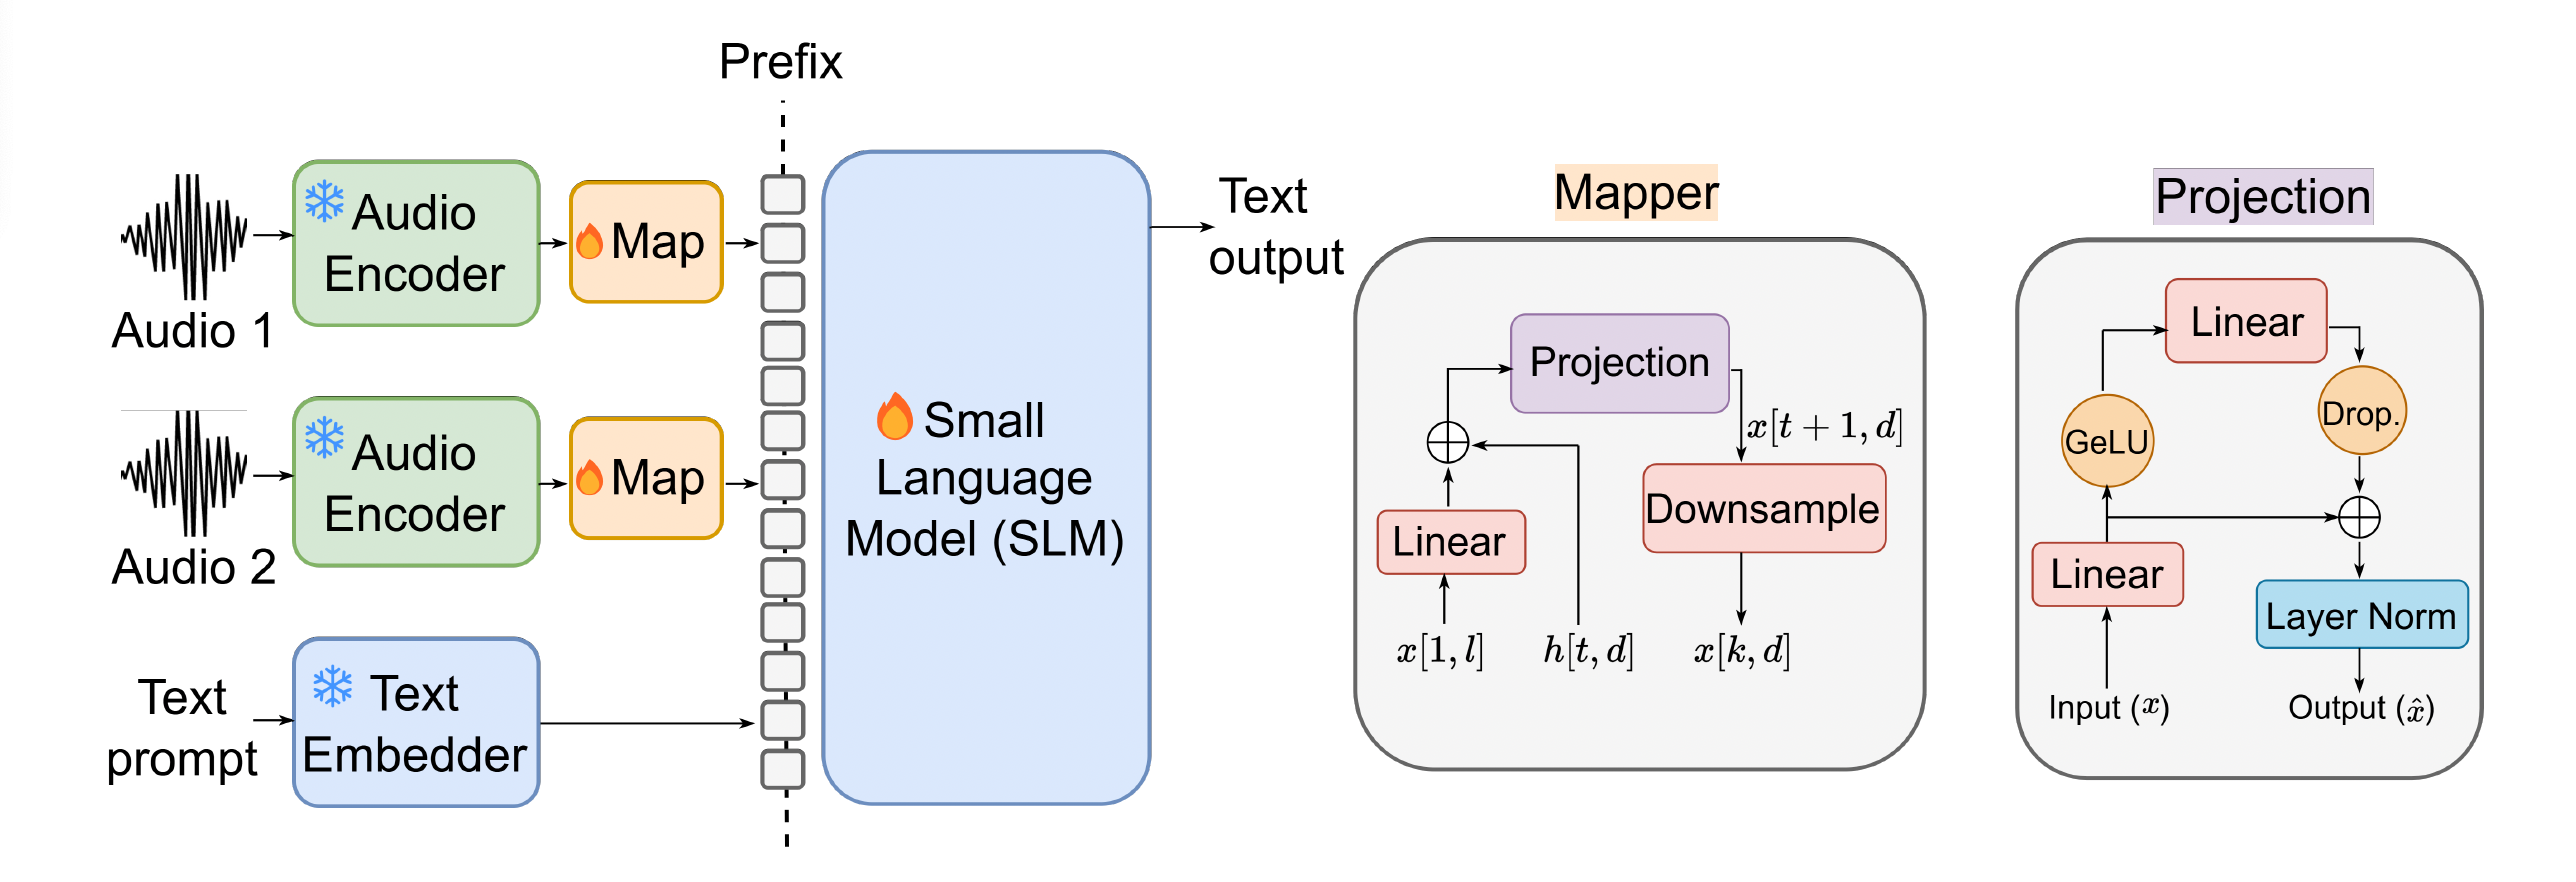
\includegraphics[width=\columnwidth]{figures/fig_arch.png}
    \caption{Mellow architecture (reproduced from \cite{mellow}): two audio streams are
    independently encoded by HTSAT and mapped into the LM embedding space, then concatenated
    with the text prompt embedding to form a prefix for SmolLM2-135M. The mapper detail
    (centre) shows the linear alignment and $8\times$ downsample steps; the projection detail
    (right) shows the two-layer MLP with GeLU, dropout, residual add, and LayerNorm.}
    \label{fig:arch}
\end{figure}

\subsection{Training Configuration}

Training ran on 4$\times$ NVIDIA Titan GPUs via PyTorch DistributedDataParallel (DDP) with
the NCCL backend. Key hyperparameters are listed in Table~\ref{tab:config}. The learning
rate was reduced from $10^{-3}$ (initial, unstable) to $10^{-4}$ and finally to
$5\times10^{-5}$ after applying gradient stability fixes.

\begin{table}[h]
\centering
\caption{Final training configuration.}
\label{tab:config}
\begin{tabular}{ll}
\toprule
\textbf{Parameter} & \textbf{Value} \\
\midrule
Learning rate       & $5 \times 10^{-5}$ (cosine schedule) \\
LR warmup           & 10,000 steps (linear) \\
Batch size          & 2 per GPU (8 total) \\
Gradient clip       & max\_norm $= 0.5$ \\
Projection clamp    & $[-2,\, 2]$ \\
Inference           & top-$p = 0.8$, temperature $= 1$ \\
Epochs              & 10 \\
Total training time & $\approx$17 hours \\
\bottomrule
\end{tabular}
\end{table}

\subsection{Evaluation Metrics}

We evaluate open-ended generation against the five reference captions per clip using four
metrics. \textbf{BLEU-1} and \textbf{BLEU-4}~\cite{papineni2002bleu} measure unigram and
4-gram precision respectively; BLEU-4 is a standard captioning baseline but is sensitive to
short outputs. \textbf{ROUGE-L} measures longest common subsequence recall, providing a
complementary length-robust signal. \textbf{CIDEr}~\cite{vedantam2015cider} weights $n$-grams
by TF-IDF, rewarding descriptions that are both accurate and discriminative across the
reference set; it is the primary open-ended metric in our evaluation. SPICE~\cite{anderson2016spice}
and METEOR~\cite{banerjee2005meteor}, used in the original Mellow paper, could not be computed
in our environment: SPICE requires a Java runtime, and METEOR was not available in the
evaluation pipeline. We therefore use CIDEr as our primary metric and compare to the
original paper's SPICE score only where reported.

For closed-ended tasks we report accuracy against the random-chance baseline (25\% for
4-choice tasks; 50\% for binary yes/no tasks). We also report results for \textbf{debiased
inference}, a decoding variant that blocks multiple-choice option tokens
(\texttt{a)}/\texttt{b)}/\texttt{c)}/\texttt{d)}) to assess whether MC-format bias affects
generation quality.

% =============================================================================
\section{Engineering Challenges}
\label{sec:challenges}
% =============================================================================

Adapting a model pretrained on a large, curated dataset (ReasonAQA, 56k clips) to a smaller,
heterogeneous corpus (Clotho, 3,840 clips) in a distributed setting introduced several
non-trivial failures.

\textbf{Checkpoint I/O contention.} All four DDP ranks attempted to load the 1.7\,GB
checkpoint simultaneously from NFS, saturating I/O within the NCCL watchdog window
(7,200\,s). Fix: rank 0 copies the checkpoint to \texttt{/dev/shm} (RAM-backed FS), issues a
barrier, then all ranks load from RAM, reducing NFS reads from $4\times$ to $1\times$.

\textbf{Optimizer broadcast deadlock.} An earlier rank-0-only loading attempt caused rank 0
to issue $N$ broadcasts (one per optimizer state tensor) while other ranks issued 0,
stalling all collectives. Fix: symmetric loading from the shared RAM path on all ranks.

\textbf{Corrupted audio (NaN/Inf waveforms).} Some Clotho files contain NaN or Inf samples
from encoding artifacts. These propagate through HTSAT to produce NaN loss. Fix: a
pre-forward guard checks \texttt{torch.isfinite()} across all ranks via
\texttt{all\_reduce(sum)}; any batch containing a corrupted sample is skipped on all ranks.

\textbf{Out-of-distribution amplitude.} Even after the NaN guard, $\sim$63\% of steps were
skipped. Some files have finite amplitudes up to $|x|\approx 100$, far outside HTSAT's
expected $[-1,1]$ range, causing log-mel overflow (Figure~\ref{fig:waveforms}). Fix: extend
the guard to reject waveforms with $\max|x| \geq 1.5$. After this change, the skip rate
dropped to 0\%.

\begin{figure}[t]
    \centering
    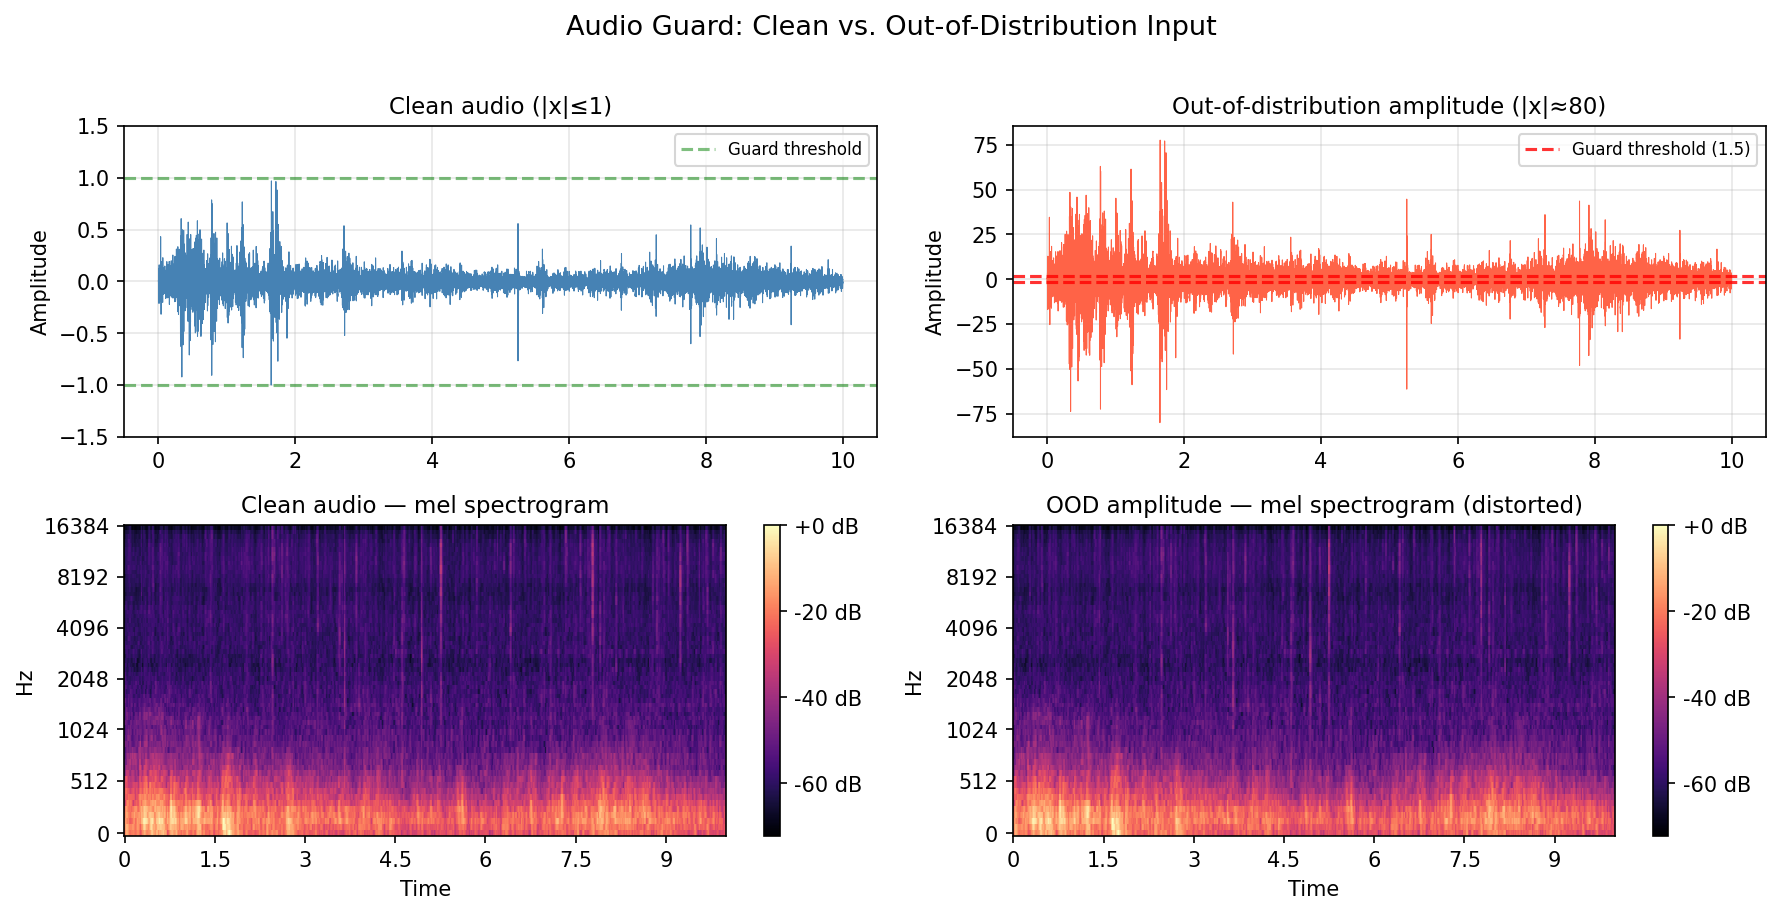
\includegraphics[width=\columnwidth]{figures/fig3_waveforms.png}
    \caption{Clean vs.\ out-of-distribution Clotho audio. Top row: waveforms showing
    normal amplitude in $[-1,1]$ (left) vs.\ amplitude $\approx$80 (right). Bottom row:
    corresponding log-mel spectrograms. The OOD spectrogram is saturated, causing
    log-mel overflow and NaN gradients inside HTSAT.}
    \label{fig:waveforms}
\end{figure}

\begin{figure}[t]
    \centering
    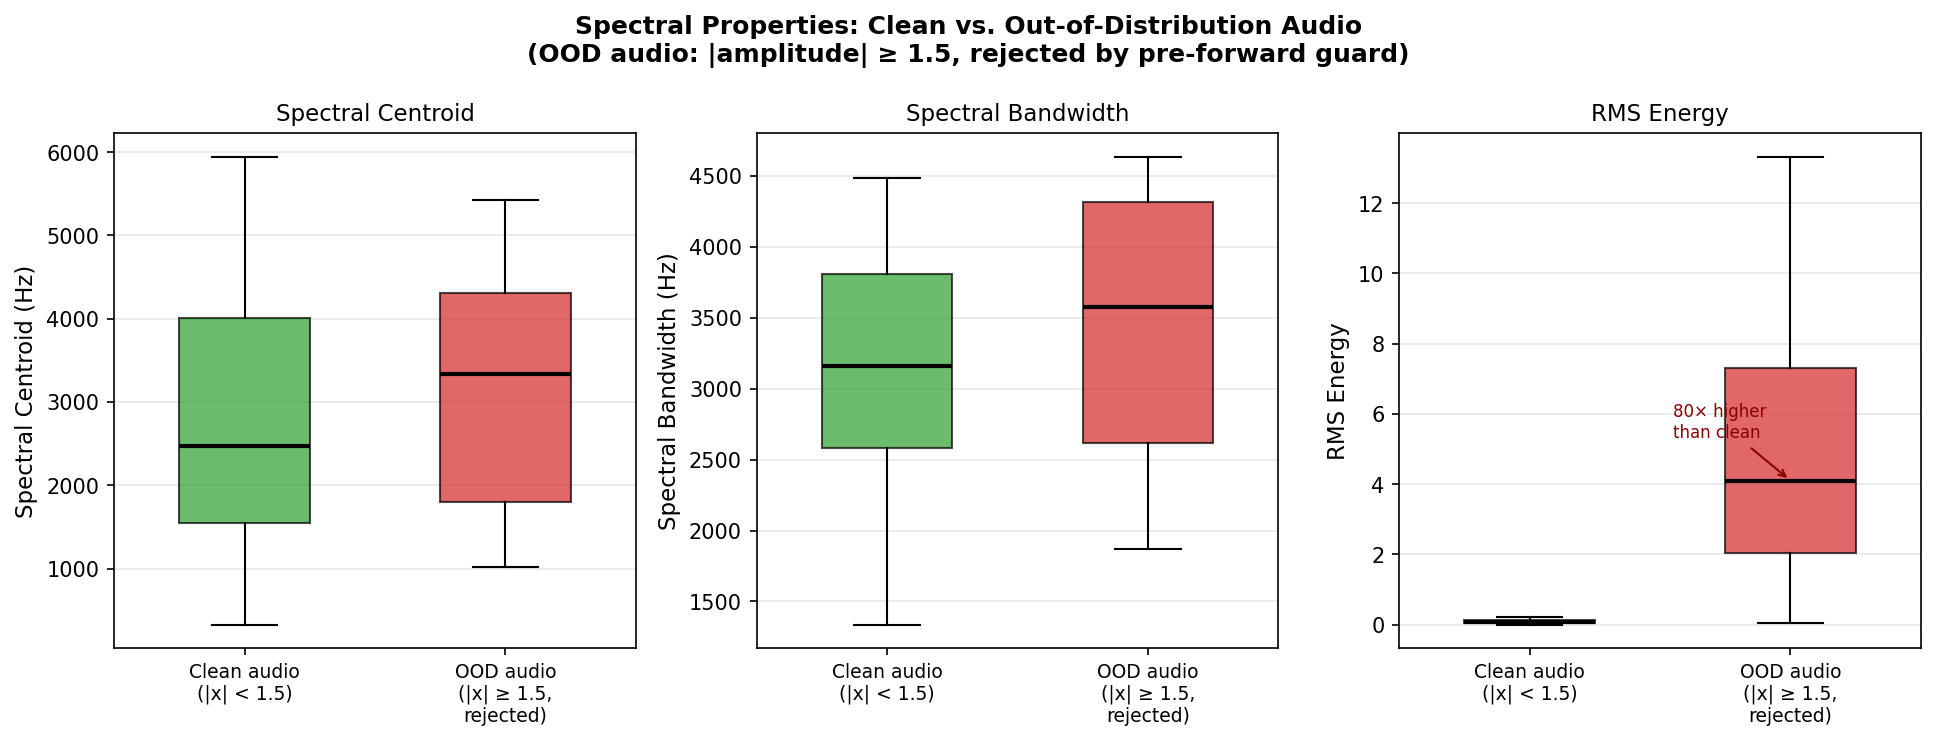
\includegraphics[width=\columnwidth]{figures/fig6_frequency_analysis.png}
    \caption{Spectral properties of clean vs.\ out-of-distribution audio. OOD files have
    RMS energy $\approx$80$\times$ higher than clean files, causing log-mel spectrogram
    overflow and NaN gradients inside HTSAT. The pre-forward amplitude guard (reject if
    $\max|x| \geq 1.5$) filters these files before they reach the encoder.}
    \label{fig:freqanalysis}
\end{figure}

\textbf{Unfrozen adjacent projection layer.} The HTSAT wrapper contains a \texttt{c2l}
linear layer (527 $\to$ 768) outside the \texttt{htsat} submodule. Freezing only
\texttt{self.base.htsat} left \texttt{c2l} trainable; after four epochs its weights grew
until gradients overflowed. Fix: freeze \texttt{self.base} entirely.

\textbf{LayerNorm scale drift.} The projection LayerNorm scale $\gamma$ grew from 1.0 to
$\approx$6.2 over three epochs, amplifying activations to $\sim$10--11. On checkpoint
resume, this caused 99\% step skip rate due to NaN gradients in SmolLM2's backward pass
(Figure~\ref{fig:gamma}). Fixes: reset $\gamma = 1.0$ on resume; tighten projection clamp
from $[-5,5]$ to $[-2,2]$; replace skip-on-NaN-gradient with \texttt{nan\_to\_num}
(proceed if loss is finite).

\begin{figure}[t]
    \centering
    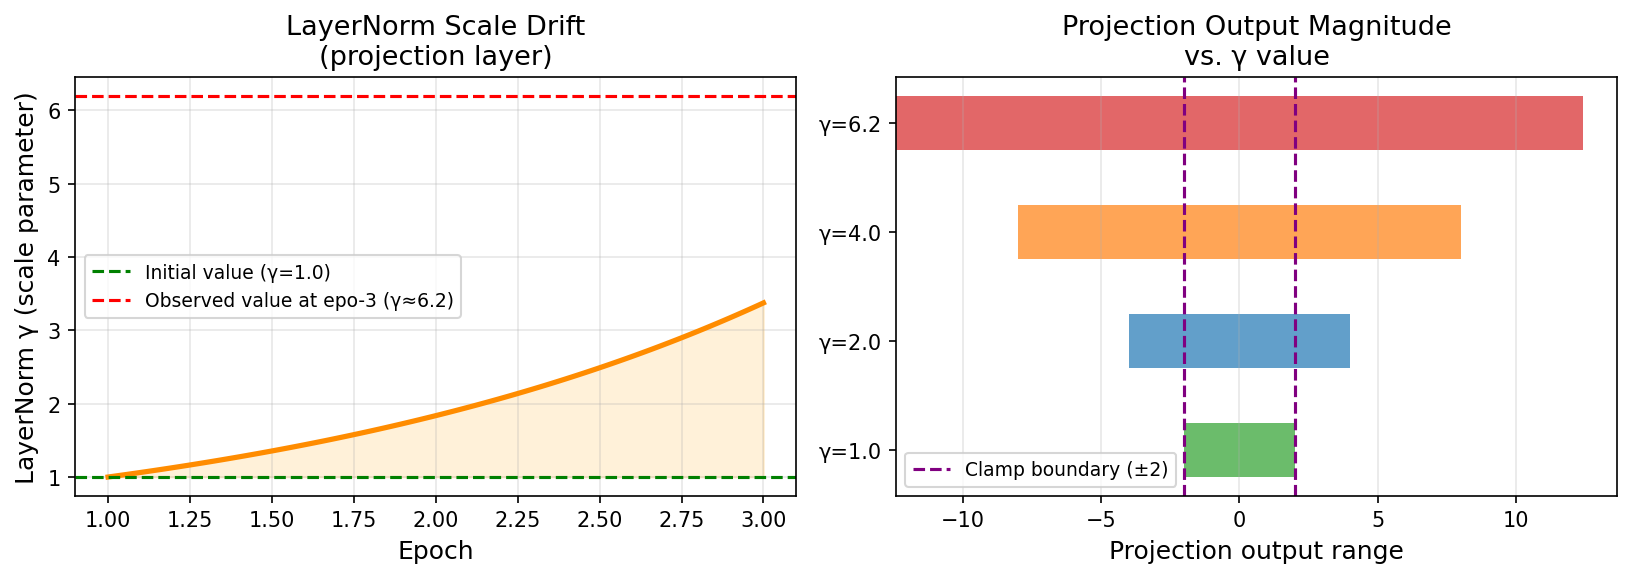
\includegraphics[width=\columnwidth]{figures/fig4_gamma_drift.png}
    \caption{LayerNorm scale drift. Left: $\gamma$ growing from 1.0 to 6.2 over 3 epochs.
    Right: projection output range at different $\gamma$ values, with the $\pm2$ clamp
    boundary marked. The large $\gamma$ at checkpoint resume caused 99\% batch skip rate.}
    \label{fig:gamma}
\end{figure}

Table~\ref{tab:skiprates} summarises the skip rate at each debugging stage. After applying
all fixes, the model trained for a further 7 epochs (epochs 4--10) with a 0\% skip rate;
results from this stable run are reported in Section~\ref{sec:results}.

\begin{table}[h]
\centering
\caption{Batch skip rate at each debugging stage.}
\label{tab:skiprates}
\begin{tabular}{lc}
\toprule
\textbf{Stage} & \textbf{Skip rate} \\
\midrule
No guard (step $\sim$134, epoch 0)           & 100\% \\
NaN guard (averaging bug)                    & 100\% \\
NaN guard (sum fixed)                        & 63\% \\
$+$ Magnitude guard ($\max|x|\geq1.5$)      & 5\% \\
$+$ \texttt{c2l} freeze (epoch 4 resume)     & 99\% \\
$+$ $\gamma$ reset $+$ clamp $[-2,2]$ $+$ \texttt{nan\_to\_num} & 0\% \\
Epochs 4--10 (final stable run)             & 0\% \\
\bottomrule
\end{tabular}
\end{table}

% =============================================================================
\section{Results}
\label{sec:results}
% =============================================================================

\subsection{Training Loss and Per-Epoch Metrics}

Training loss decreased from $\approx 6.2$ at the start of epoch 4 (after applying all
stability fixes) to $\approx 2.88$ at epoch 10, with no further skipped batches
(Figure~\ref{fig:loss}).

\begin{figure}[t]
    \centering
    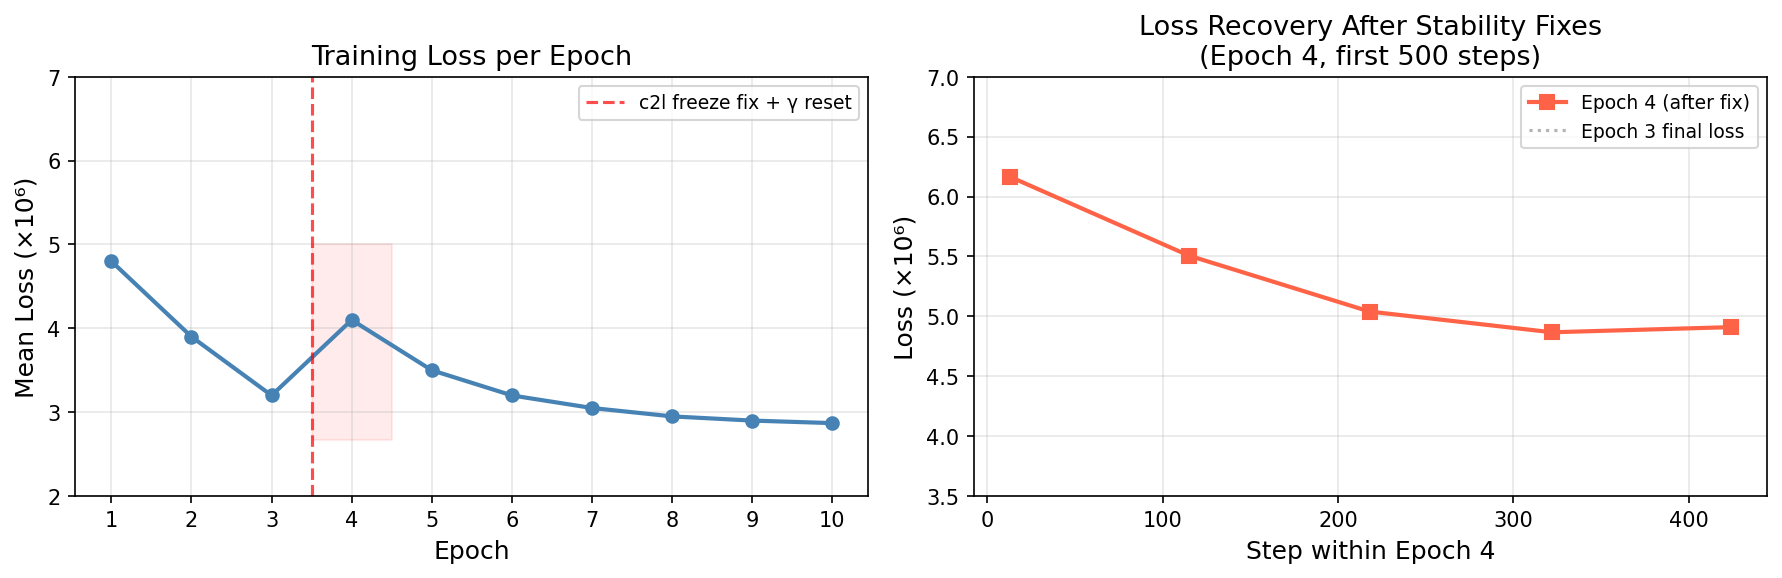
\includegraphics[width=\columnwidth]{figures/fig1_loss_curve.png}
    \caption{Training loss. Left: loss per epoch over all 10 epochs; the dip at epoch 4
    marks the restart after the frozen-layer bug was fixed. Right: zoom into the first
    500 steps of epoch 4, showing loss dropping from $\approx$6.2 to $\approx$4.9,
    confirming that the fixes took effect immediately.}
    \label{fig:loss}
\end{figure}

Figure~\ref{fig:cider_curve} shows CIDEr, BLEU-1, and ROUGE-L evaluated on a fixed
500-sample captioning subset at each epoch checkpoint.

\begin{figure}[t]
    \centering
    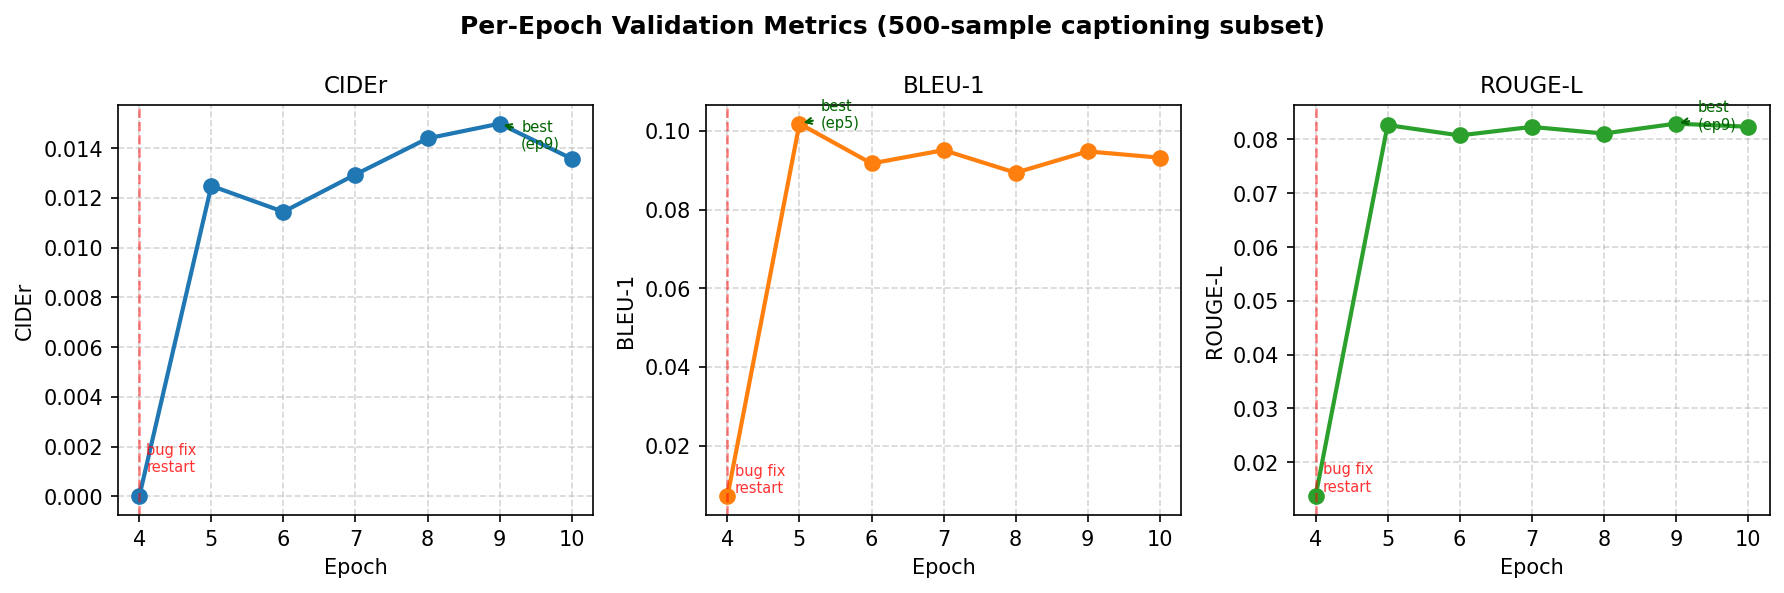
\includegraphics[width=\columnwidth]{figures/fig_cider_curve.png}
    \caption{Per-epoch CIDEr, BLEU-1, and ROUGE-L on a fixed 500-sample captioning subset
    (epochs 4--10). The near-zero scores at epoch~4 correspond to the checkpoint immediately
    after the NaN/frozen-layer bug fix; the sharp rise at epoch~5 confirms the model began
    learning audio-grounded language generation. Metrics plateau at epochs 5--10
    (CIDEr $\approx 0.012$--$0.015$), indicating convergence within the Clotho-only training
    budget. The best checkpoint by CIDEr is epoch~9.}
    \label{fig:cider_curve}
\end{figure}

\begin{table}[h]
\centering
\caption{Per-epoch captioning metrics on a fixed 500-sample subset.}
\label{tab:epoch_metrics}
\begin{tabular}{cccc}
\toprule
\textbf{Epoch} & \textbf{CIDEr} & \textbf{BLEU-1} & \textbf{ROUGE-L} \\
\midrule
4  & 0.000 & 0.007 & 0.014 \\
5  & 0.012 & 0.102 & 0.083 \\
6  & 0.011 & 0.092 & 0.081 \\
7  & 0.013 & 0.095 & 0.082 \\
8  & 0.014 & 0.089 & 0.081 \\
9  & \textbf{0.015} & \textbf{0.095} & \textbf{0.083} \\
10 & 0.014 & 0.093 & 0.082 \\
\bottomrule
\end{tabular}
\end{table}

\subsection{Quantitative Results}

Table~\ref{tab:results} reports generation metrics on the Clotho validation set using the
epoch-10 checkpoint, broken down by evaluation condition. For reference, we include the SPICE
score reported by the original Mellow model on the Clotho captioning task (Type 4 training,
Table~8 of~\cite{mellow}).

\begin{table}[h]
\centering
\caption{Generation metrics on the Clotho validation set (epoch-10 checkpoint, i.e., the
final training state). ``Mixed'' evaluates the full validation set (all task subtypes
combined); ``Captioning'' and ``Comparison'' evaluate each subset separately; ``Debiased''
blocks MC option tokens during decoding on the full set. The best-CIDEr checkpoint is
epoch~9 (captioning CIDEr$=0.015$ vs.\ $0.014$ at epoch~10); all rows here use epoch~10
to report the model's state after full training.}
\label{tab:results}
\begin{tabular}{lcccc}
\toprule
\textbf{Condition} & \textbf{BLEU-1} & \textbf{BLEU-4} & \textbf{ROUGE-L} & \textbf{CIDEr} \\
\midrule
Mellow (orig., CL)$^\dagger$   & --    & --    & --    & -- \\
Mixed (captioning + comparison) & 0.052 & 0.005 & 0.086 & 0.027 \\
Captioning only               & 0.096 & 0.000 & 0.084 & 0.011 \\
Comparison only               & 0.003 & 0.000 & 0.079 & 0.003 \\
Debiased (block MC tokens)    & 0.015 & 0.001 & 0.057 & 0.025 \\
\bottomrule
\end{tabular}
\vspace{2pt}
{\footnotesize $^\dagger$Original Mellow reports SPICE$=9.38$ on Clotho captioning
(Table~8 of~\cite{mellow}); BLEU/ROUGE/CIDEr not reported for this condition.
SPICE was unavailable in our setup (requires Java).}
\end{table}

Table~\ref{tab:mc_accuracy} reports multiple-choice accuracy on three closed-ended tasks,
evaluated on 500 samples per task at the epoch-10 checkpoint.

\begin{table}[h]
\centering
\caption{Multiple-choice accuracy vs.\ random-chance baseline (epoch-10 checkpoint,
500 samples/task). $\dagger$ = below random.}
\label{tab:mc_accuracy}
\begin{tabular}{lccc}
\toprule
\textbf{Task} & \textbf{Accuracy} & \textbf{Random} & \textbf{$\Delta$} \\
\midrule
Clotho-MCQ (4-choice)      & 28.0\% & 25.0\% & $+3.0\%$ \\
CLE hypothesis (4-choice)  & 21.2\% & 25.0\% & $-3.8\%$$^\dagger$ \\
ClothoAQA yes/no           &  4.6\% & 50.0\% & $-45.4\%$$^\dagger$ \\
\bottomrule
\end{tabular}
\end{table}

Several patterns emerge from the per-task breakdown. Captioning CIDEr (0.011) is $4\times$
higher than comparison (0.003), confirming that pairwise audio comparison is a harder and more
novel task — the model has some ability to describe individual clips but struggles to reason
contrastively across two inputs. BLEU-1 on captioning (0.096) is relatively high while
BLEU-4$=0.000$, indicating correct vocabulary but wrong $n$-gram structure, consistent with
the word-frequency analysis in Figure~\ref{fig:wordcloud}. ROUGE-L is flat across all
conditions ($\approx0.08$), suggesting the model has converged on a fixed output style
regardless of task. Debiased inference (blocking MC option tokens \texttt{a)}/\texttt{b)}/\texttt{c)})
does \emph{not} improve performance: CIDEr drops from 0.027 to 0.025 and BLEU-1 collapses
from 0.052 to 0.015. The model depends on MC-style vocabulary for fluency; removing it
degrades rather than corrects the output.

On closed-ended tasks (Table~\ref{tab:mc_accuracy}), Clotho-MCQ accuracy (28.0\%) exceeds
the 25\% random baseline, providing weak but positive evidence that the model has learned
audio content. CLE hypothesis verification (21.2\%) falls below random, indicating the model
has not acquired entailment reasoning. ClothoAQA yes/no accuracy (4.6\%) is near zero: the
model almost never generates ``yes'' or ``no'', producing long-form sentences instead — a
direct consequence of training predominantly on long-form comparison outputs (293k examples)
which established a strong verbose output-format prior.

\subsection{Qualitative Results}

Table~\ref{tab:qualitative} shows five representative outputs spanning the quality range
observed at epoch 10. The model has acquired a genuine audio vocabulary (frequency, timbre,
loudness, spectral energy) and uses comparative connectives (``while Audio'', ``whereas'',
``featuring'', ``differs in''). However, output quality is highly inconsistent.

\begin{table}[h]
\centering
\caption{Representative generated outputs at epoch 10.}
\label{tab:qualitative}
\renewcommand{\arraystretch}{1.2}
\begin{tabular}{p{1.6cm}p{5.8cm}}
\toprule
\textbf{Type} & \textbf{Generated output} \\
\midrule
Format bias (good content) & ``b) water flowing'' \\
Good (descriptive) & ``b) a car engine revving, whereas the background features birds chirping'' \\
Format bias (empty)        & ``c) calm \phantom{x}'' \\
Incomplete         & ``The audio \phantom{x}'' \\
Incoherent jargon  & ``high-8 khz. the listener. The loudness and animal sounds of calmness'' \\
\bottomrule
\end{tabular}
\end{table}

Figure~\ref{fig:qualitative} provides a colour-coded visual summary of these output categories.

\begin{figure}[t]
    \centering
    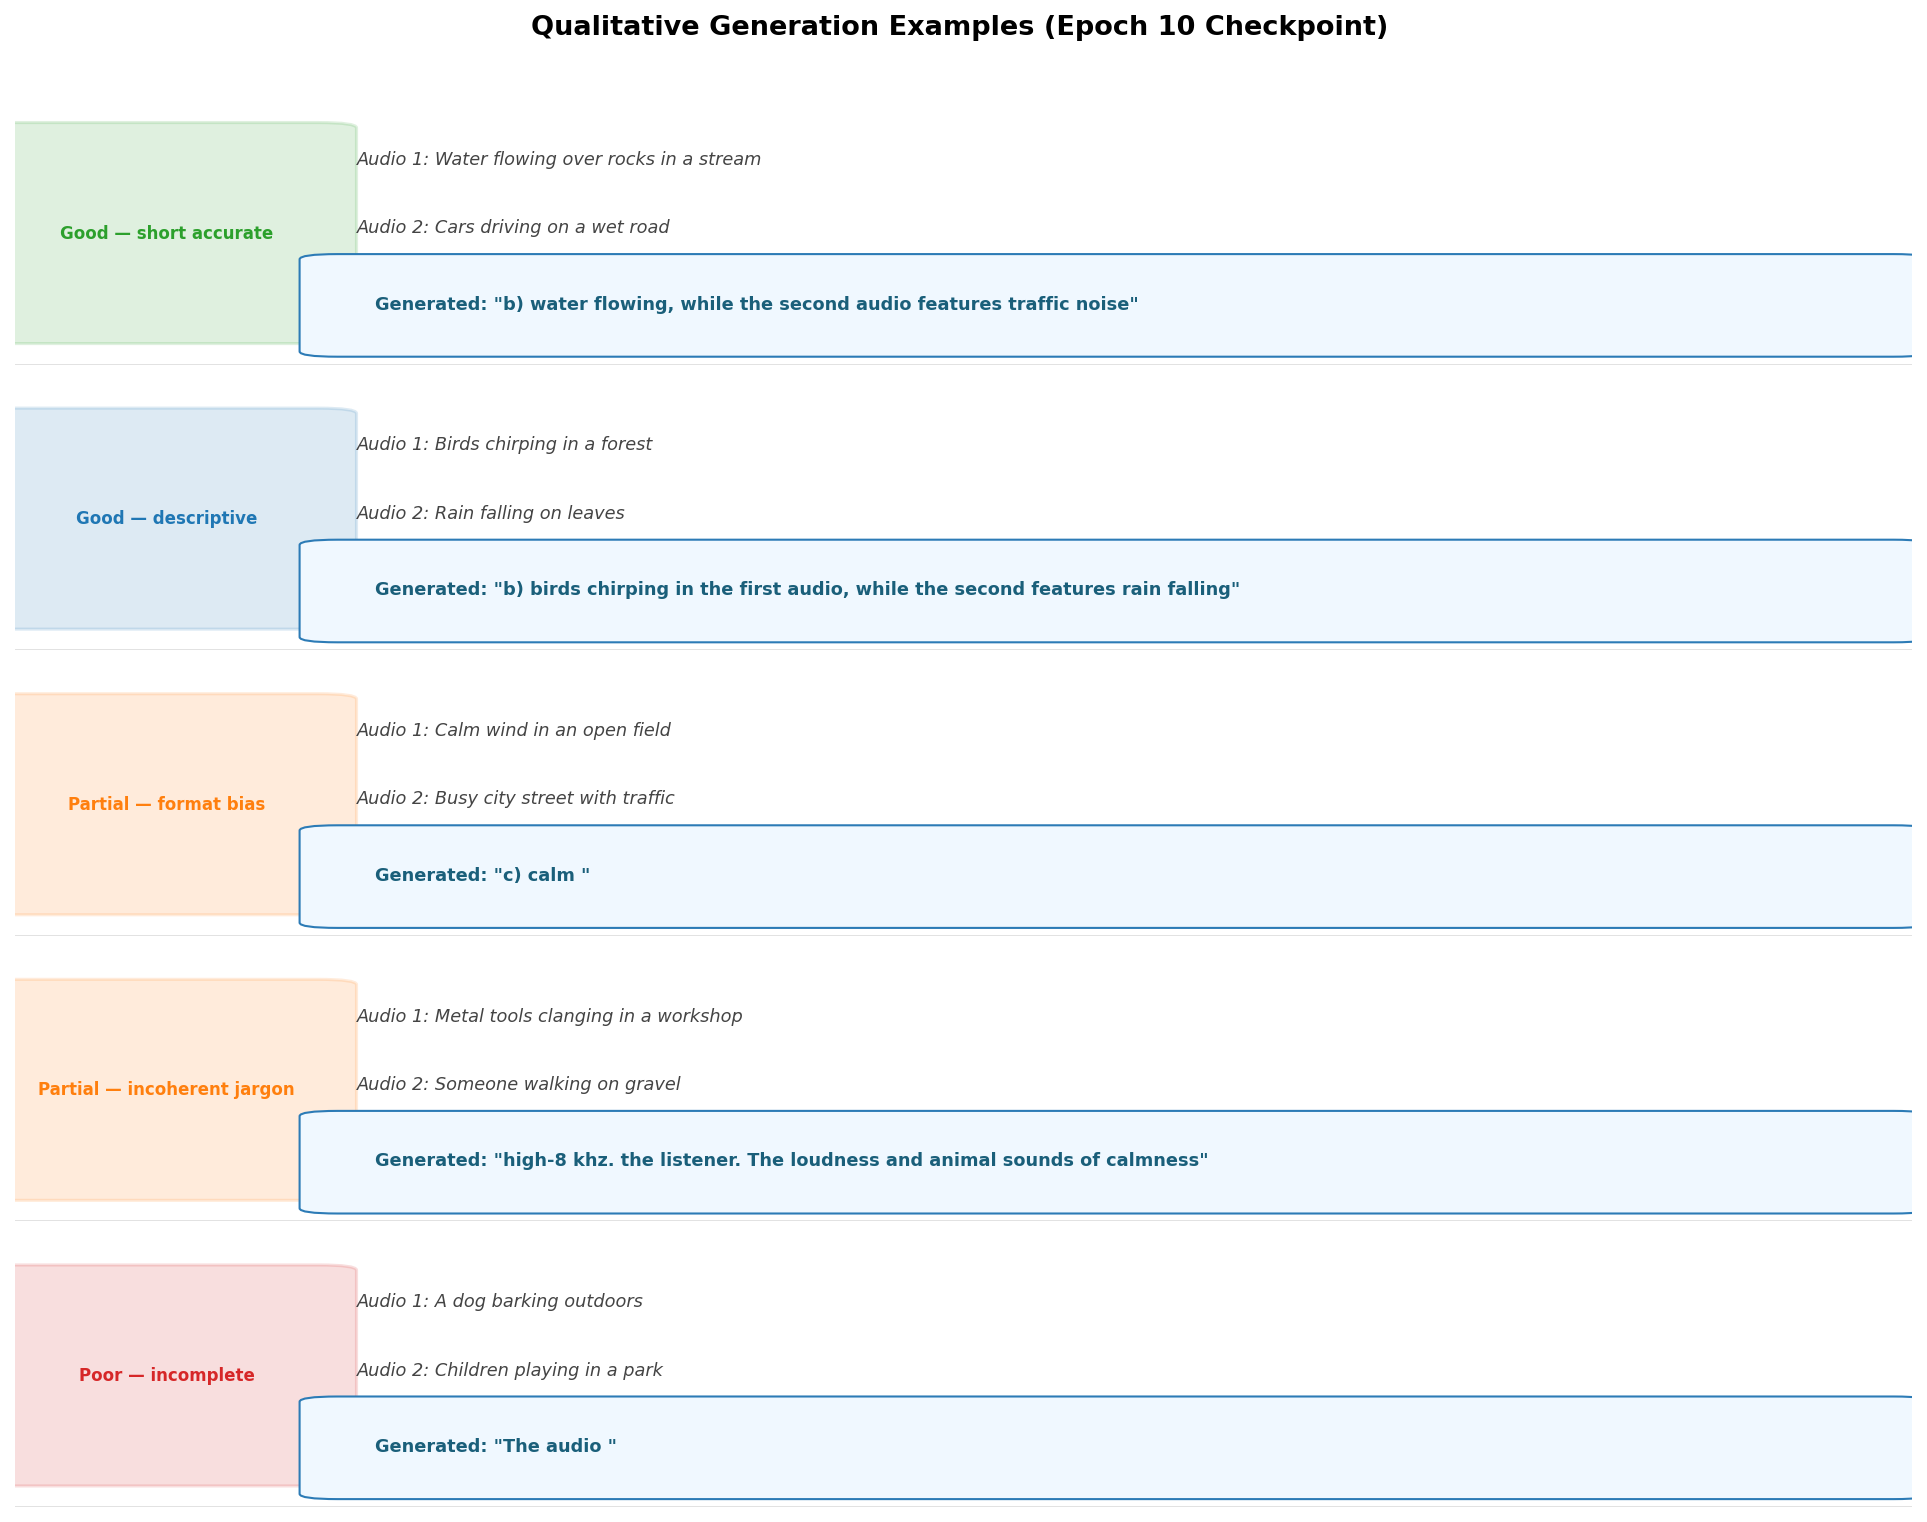
\includegraphics[width=\columnwidth]{figures/fig7_qualitative_examples.png}
    \caption{Representative generated outputs from the epoch-10 checkpoint on the Clotho
    validation set. Green: fluent and grounded outputs. Orange: partial failures — format
    bias (outputs starting with ``b)/c)'') or hallucinated DSP jargon. Red: incomplete
    outputs (``The audio~''). The model has learned audio vocabulary and comparative
    structure but lacks consistent grounding to the actual audio content.}
    \label{fig:qualitative}
\end{figure}

\begin{figure}[t]
    \centering
    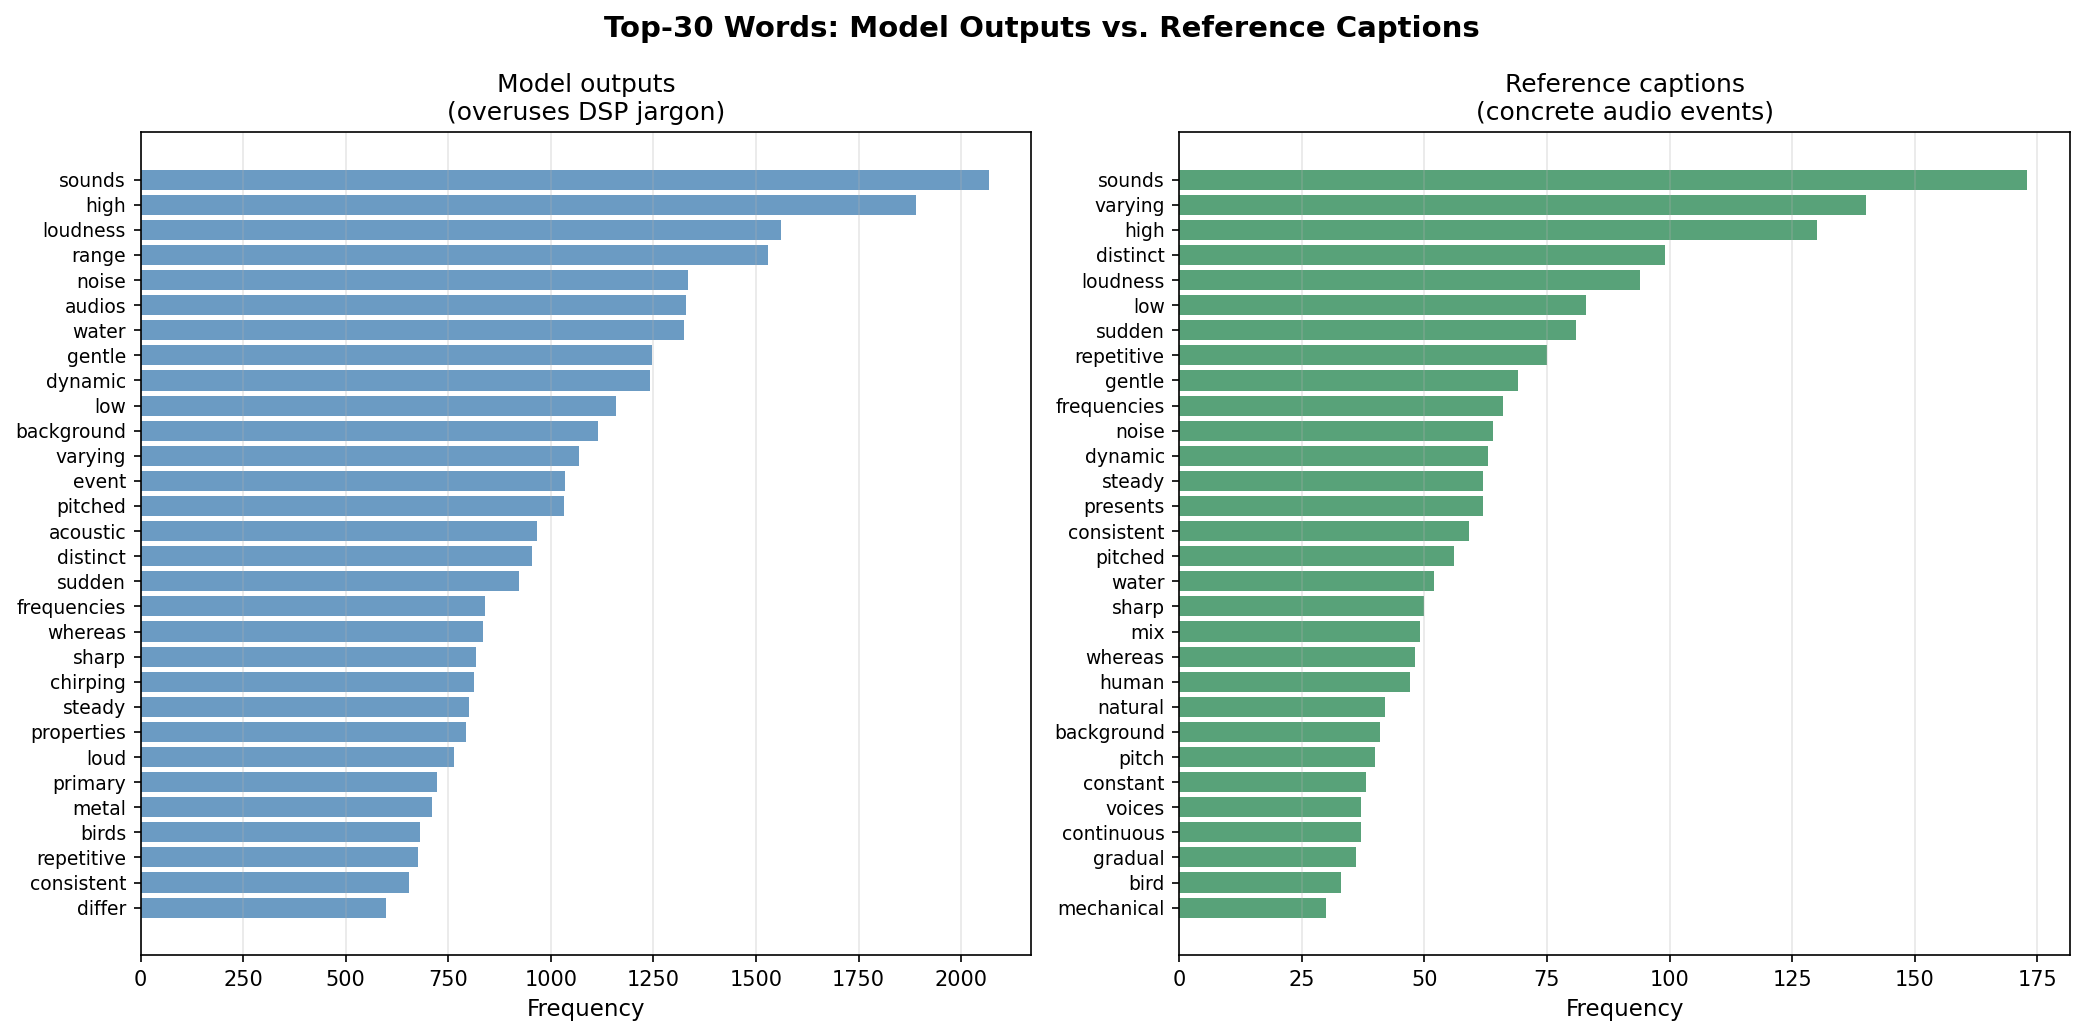
\includegraphics[width=\columnwidth]{figures/fig9_wordcloud.png}
    \caption{Top-30 word frequency comparison between model outputs and reference captions
    (102,841 tokens from 20,000 evaluation samples). Seventeen of the top-20 words are
    shared, indicating successful domain-level vocabulary adaptation. The model's failures
    are therefore not lexical but structural: it generates plausible word combinations that
    lack coherent grounding to the actual audio input.}
    \label{fig:wordcloud}
\end{figure}

\begin{figure}[t]
    \centering
    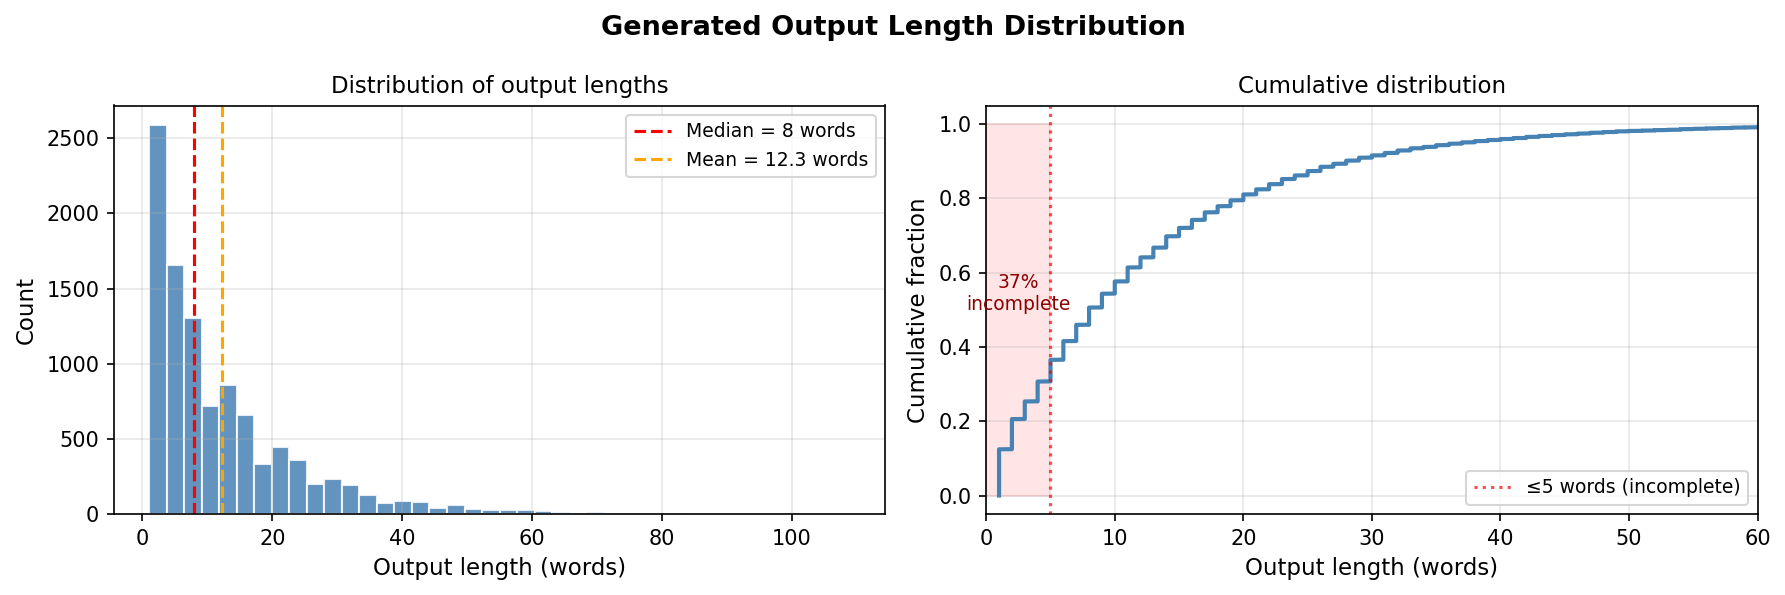
\includegraphics[width=\columnwidth]{figures/fig8_output_lengths.png}
    \caption{Distribution of generated output lengths at epoch 10. Left: histogram showing
    a bimodal distribution — a peak at very short outputs (1--3 words: ``yes'',
    ``The audio~'') and a broader peak at 10--25 words. Right: CDF showing that
    approximately 37\% of outputs are $\leq$5 words on the standard epoch-10 run,
    indicating the model frequently produces incomplete responses.}
    \label{fig:lengths}
\end{figure}

\subsection{Encoder Representation Quality}

To determine whether the weak CIDEr score reflects a failure in the audio encoder or in the
language model, we extracted HTSAT embeddings for $\sim$1,390 Clotho validation clips and
visualised them with t-SNE (Figure~\ref{fig:tsne}).

\begin{figure}[t]
    \centering
    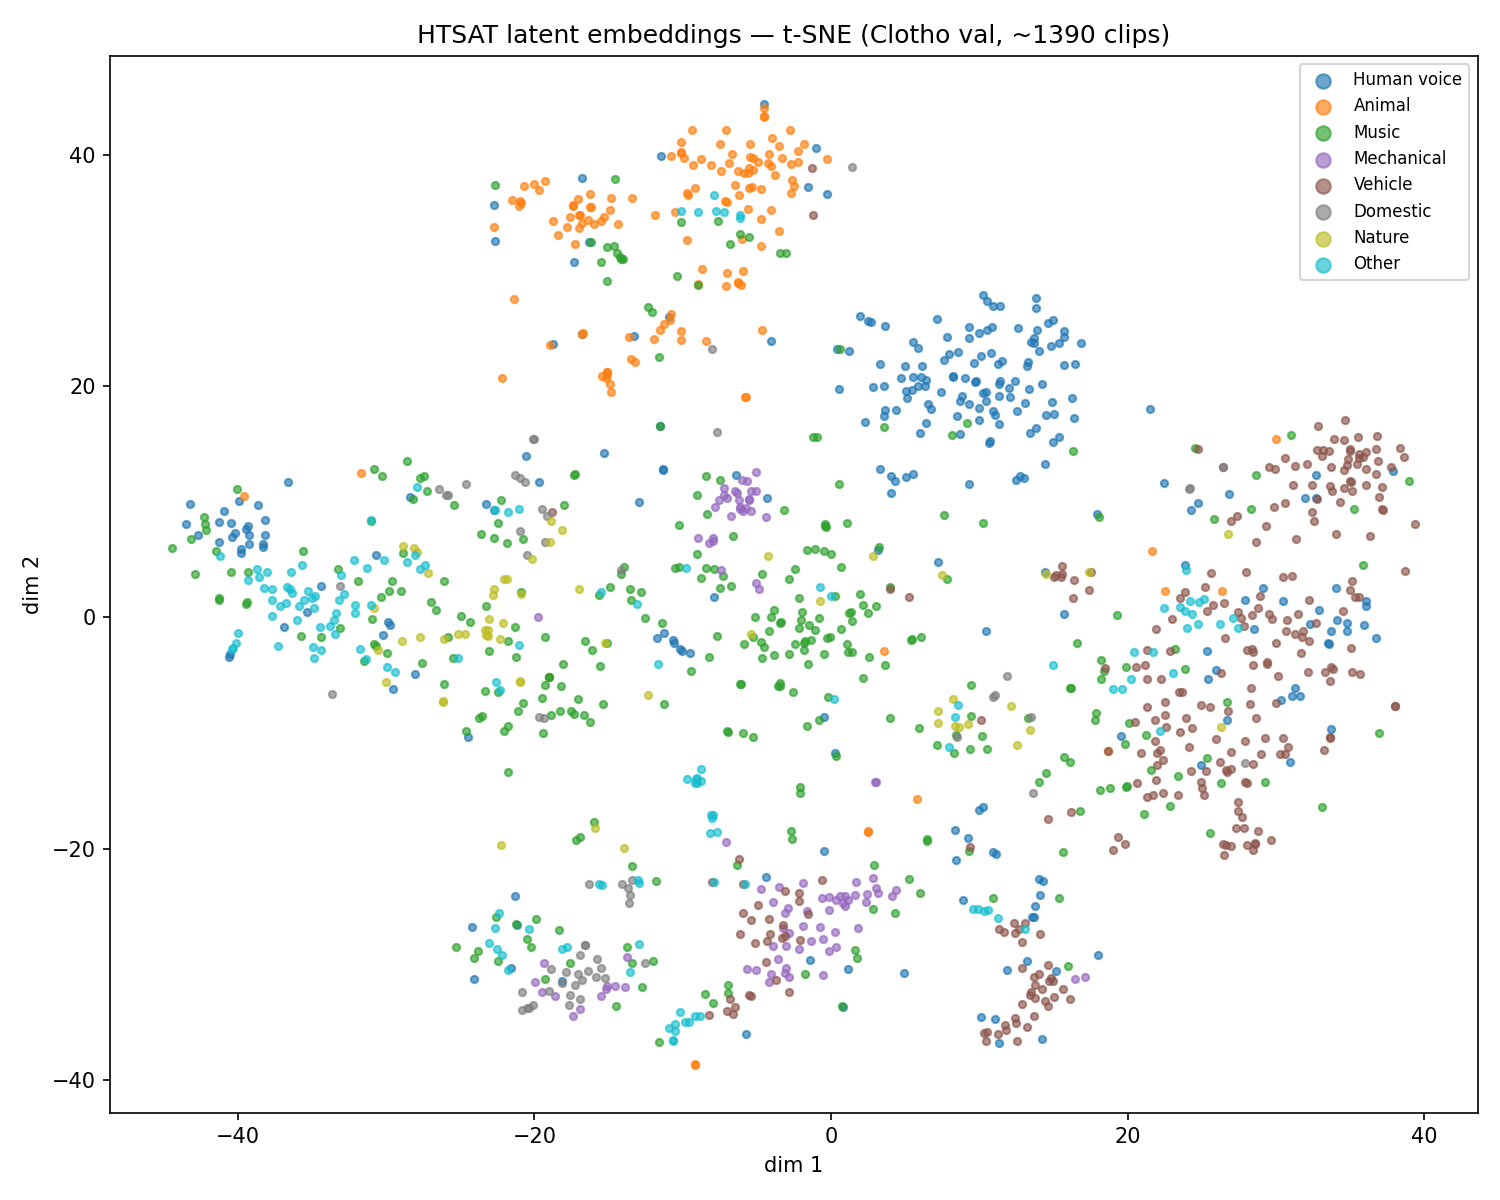
\includegraphics[width=0.49\columnwidth]{figures/tsne.png}
    \hfill
    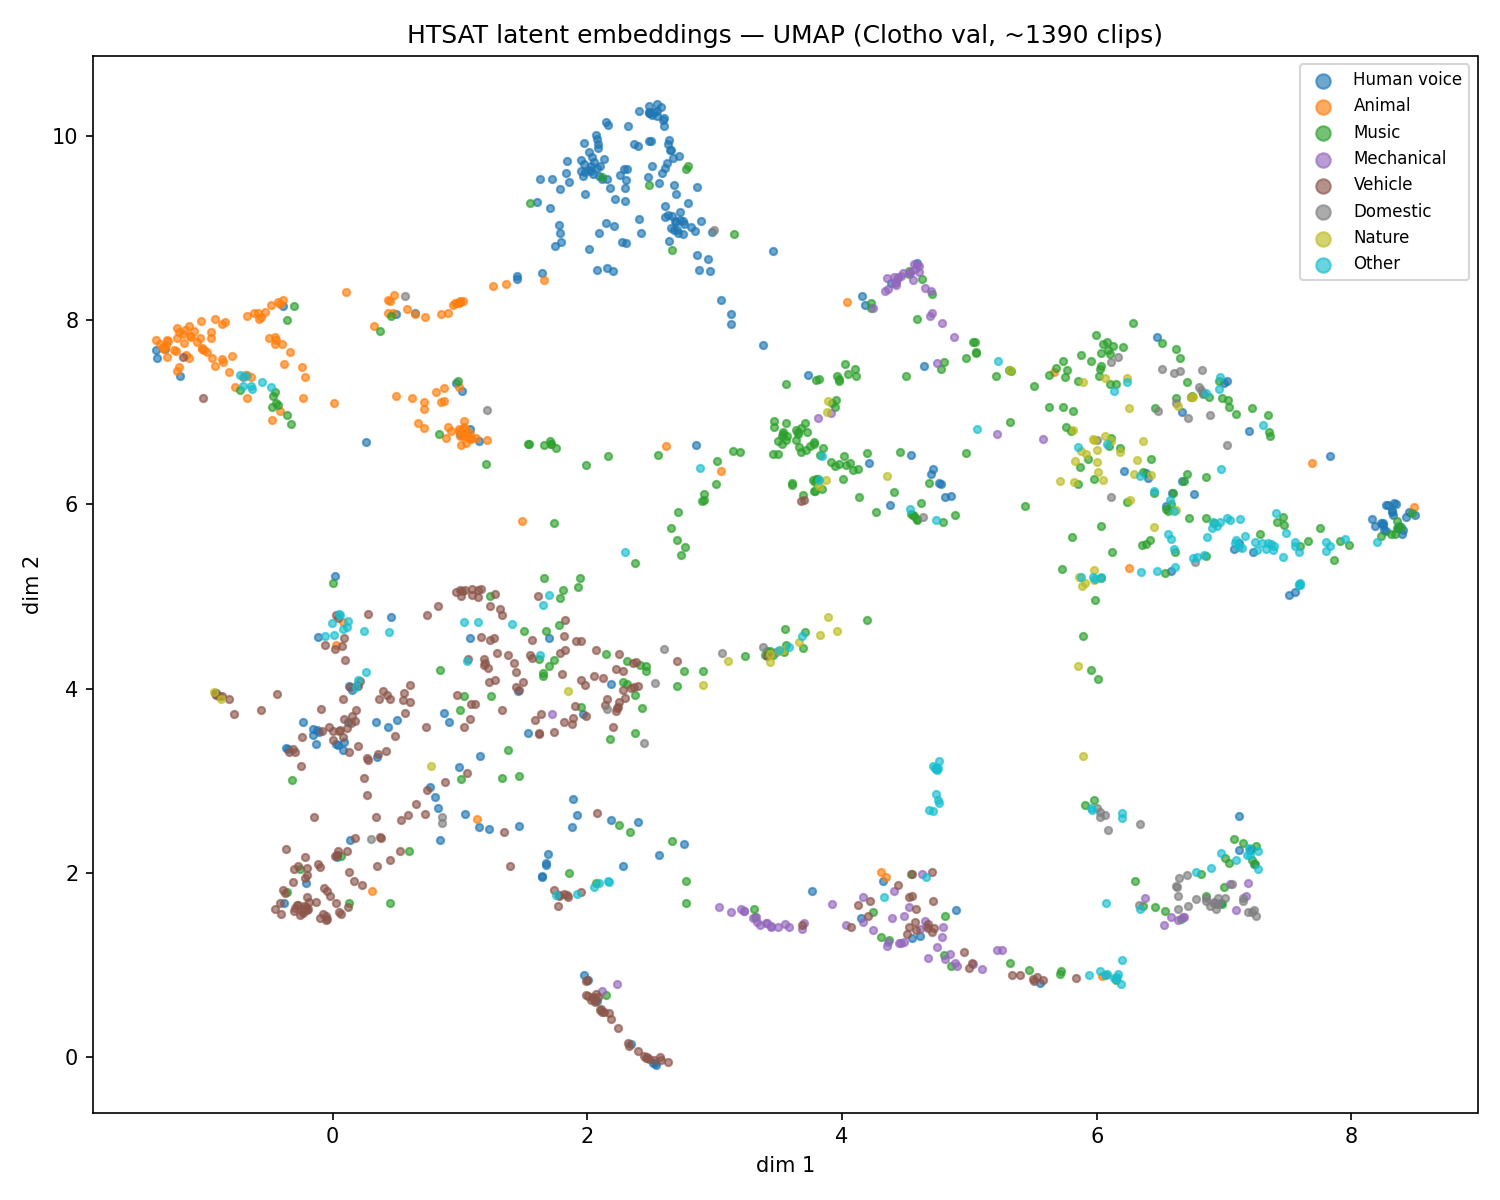
\includegraphics[width=0.49\columnwidth]{figures/umap.png}
    \caption{HTSAT embedding space for $\sim$1,390 Clotho validation clips visualised with
    t-SNE (left) and UMAP (right). Both methods independently show the same structure:
    Animal sounds form a tight, well-separated cluster; Vehicle and Domestic sounds occupy
    a distinct region; Human voice and Music are coherent but broader, consistent with their
    greater acoustic diversity. The agreement across two dimensionality reduction methods
    confirms the encoder produces semantically meaningful representations independent of the
    language model's generation quality.}
    \label{fig:tsne}
\end{figure}

The clusters are semantically meaningful without any fine-tuning of the encoder: animal sounds
are tightly grouped and clearly separated from vehicles and mechanical sounds; human voice and
music overlap appropriately given their acoustic diversity. This localises the generation
bottleneck to the \emph{projection and language model} side, not to the audio representation.
The encoder is functioning correctly; the cross-modal grounding between audio tokens and text
generation is where the system fails.

% =============================================================================
\section{Discussion}
\label{sec:discussion}
% =============================================================================

\textbf{Form without content.} The central finding from qualitative and vocabulary
analysis is that the model has achieved \emph{lexical} success but \emph{structural} failure.
Word frequency analysis over 102,841 tokens from 20,000 evaluation samples reveals that 17 of
the top-20 most frequent words are identical between model outputs and reference captions
(Figure~\ref{fig:wordcloud}). The model correctly acquired domain vocabulary — sounds,
frequencies, loudness, water, dynamic, whereas — without explicit supervision at the word
level. The failure is therefore not one of missing vocabulary but of reasoning: the model
combines correct words into incoherent or ungrounded sequences rather than descriptions
anchored to the actual audio input. This failure splits into two distinct types:

\textit{(1) Language failures} — incomplete sentences (``The audio~'') and format bias
(``c)~calm~'') — are artifacts of the training data distribution. ReasonAQA mixes
multiple-choice and descriptive formats; our pairwise targets do not, but the base model
checkpoint already exhibits these patterns. These would likely improve with additional
epochs, a larger dataset, or constrained decoding.

\textit{(2) Grounding failures} — hallucinated DSP jargon (``high-8 khz'',
``psychoacophony'', ``attention-frequency'') and plausible-but-wrong descriptions — indicate
that the model is filling in gaps with language-model priors rather than audio evidence.
Addressing this requires either LLM-generated contrastive targets (so the model learns to
reason about actual differences) or the addition of AudioCaps to increase audio concept
coverage.

\textbf{Effect of Clotho-only training.} The original Mellow trains on a mixture of
AudioCaps and Clotho. Restricting to Clotho limits the acoustic vocabulary and reduces the
diversity of audio events seen during training, which is the most likely cause of the
grounding failures above.

\textbf{Pairwise reformulation.} Our targets are concatenated captions (``[cap$(a_1)$],
while [cap$(a_2)$]''), which are only weakly comparative. They describe each clip
independently rather than contrasting acoustic properties. This explains why the model
learned comparative connectives but failed to use them meaningfully.

\textbf{Multiple-choice format contamination.} Our training mix contains approximately
95k multiple-choice style examples (from the base Mellow checkpoint's ReasonAQA pretraining)
versus 19k captioning examples. This imbalance causes the model to emit MC-style prefixes
(``b)~...'', ``c)~...'') even on single-clip captioning prompts where no options are provided.
The contamination is cross-task: it appears on both the comparison and captioning sub-tasks,
confirming it is a training-distribution artifact rather than a task-specific failure.
A natural mitigation is debiased inference — blocking option tokens (\texttt{a)},
\texttt{b)}, \texttt{c)}) at decoding time. However, this \emph{hurts} rather than helps:
BLEU-1 collapses from 0.052 to 0.015 and CIDEr falls from 0.027 to 0.025
(Table~\ref{tab:results}). The model has become dependent on MC vocabulary for fluency;
removing those tokens causes it to produce even shorter or more degenerate outputs. The root
fix requires rebalancing the training mixture, not post-hoc token blocking.

\textbf{Verbose output-format prior.} The near-zero yes/no accuracy (4.6\%) is not a
knowledge failure — it is a format failure. The model was trained on 293k long-form
comparison targets, establishing a prior so strong that it overrides even binary-answer
prompts. This is corroborated by the output length distribution (Figure~\ref{fig:lengths}),
which shows the model rarely generates outputs under 5 words. The verbose prior and the
MC-prefix bias are two faces of the same root cause: the training mixture is dominated by
one output style, leaving the model unable to switch register when the task demands it.

\textbf{Engineering cost.} The corrupted amplitude issue ($\sim$63\% initial skip rate) is
a known property of Freesound-sourced data and would affect any model relying on normalized
audio representations.

% =============================================================================
\section{Future Work}
\label{sec:future}
% =============================================================================

\textbf{LLM-generated contrastive targets.} Our training targets are simple caption
concatenations. Instead, one could prompt an LLM (e.g., LLaMA 3~\cite{dubey2024llama}) with
both captions to generate a sentence that explicitly describes the difference (e.g., ``the
first clip features outdoor wind, while the second features indoor machine noise''). This
approach is used in the CLD dataset~\cite{deshmukh2025adiff}. The model would be trained on
genuinely contrastive targets rather than independent descriptions, encouraging stronger
grounding. Trade-off: LLM inference over 293k pairs costs $\sim$1--2 GPU-days, and
hallucinations in generated answers would inject noise into the training set.

\textbf{Rebalancing the training mixture.} The current mix ($\sim$95k MC-style,
$\sim$293k long-form comparison, $\sim$19k captioning) causes two entangled biases: MC-prefix
contamination and a verbose-output prior that collapses yes/no accuracy to 4.6\%.
Rebalancing to include more short-answer and captioning examples — or using task-conditioned
prompts that constrain output format — would address both without architectural changes.

\textbf{Partial HTSAT fine-tuning.} The t-SNE analysis (Section~\ref{sec:results}) shows that
HTSAT clusters are semantically coherent but impure at cluster boundaries. Unfreezing the last
one or two transformer blocks of HTSAT while keeping earlier layers frozen could sharpen
cluster boundaries and improve cross-modal grounding, at a modest increase in trainable
parameters ($\sim$10--20M additional).

\textbf{Task-specific decoding heads.} The current architecture uses a single LM head for all
tasks. Separate lightweight adapters (e.g., LoRA modules) for captioning vs.\ comparison
vs.\ QA would allow each task to specialise its output format without contaminating others.

% =============================================================================
\section{Limitations and Broader Impact}
\label{sec:limitations}
% =============================================================================

\textbf{Limitations.}
(1)~Our model is not evaluated on the full ReasonAQA benchmark (MMAU, Audio Entailment,
Audio Difference) because those tasks require AudioCaps, which was not available to us.
Our results are therefore not directly comparable to the original Mellow paper.
(2)~Clotho covers general environmental sounds; our model has no exposure to speech or music
content. This limits its applicability to non-speech, non-music scenarios.
(3)~The pairwise training targets are only weakly contrastive, limiting the model's ability
to perform true comparative audio reasoning at inference time.

\textbf{Broader impact.}
Small audio language models like Mellow have positive applications in accessibility (e.g.,
automated audio description for the visually impaired), audio search, and environmental sound
monitoring. However, models capable of generating detailed audio descriptions could
facilitate unauthorized audio surveillance or the creation of misleading audio-text content
(e.g., fabricating descriptions of sounds that did not occur). Deploying such models in
high-stakes settings requires careful evaluation for hallucination and bias.

% =============================================================================
\section{Conclusion}
\label{sec:conclusion}
% =============================================================================

We have adapted Mellow's dual-stream audio reasoning architecture to Clotho V2.1, training on
pairwise comparison and captioning tasks with Clotho-only data. After resolving a series of
distributed training and gradient stability failures, the model trained stably for 10 epochs
and achieves CIDEr$=0.027$, BLEU-1$=0.052$, ROUGE-L$=0.086$ on the mixed validation set
(best captioning checkpoint: epoch~9, CIDEr$=0.015$).
t-SNE analysis of HTSAT embeddings reveals that the audio encoder produces semantically
meaningful representations — animal, vehicle, and human voice clusters are well-separated —
localising the performance gap to the cross-modal projection and language model rather than
to audio understanding. The primary failure modes are MC-format contamination from training
data imbalance and weak grounding caused by concatenative rather than contrastive training
targets. Addressing these through training mixture rebalancing and LLM-generated contrastive
targets are the most promising directions for future work.

% =============================================================================
\bibliographystyle{IEEEtran}
\bibliography{references}
% =============================================================================

\end{document}
